\subsection{局部连通空间上的覆叠}

设 B 为拓扑空间，E 为 B-空间。设其投影 p 是平展且分离的映射。

若空间 B 是局部连通的，则空间 E 是局部连通的。若空间 E 是局部连通的，则 B 的开子集 \(p(\mathrm{E})\) （参看 I, p. 29, remark 2）是局部连通的。

像 \(s(\mathrm{B})\) ——这里 \(s\) 是 \(p\) 的任一截面——是开的 (I, p. 30, cor. 3) 且在 B 中是闭的 (I, p. 27, prop. 3)。若 B 是连通且非空的，则它是 E 的一个连通分支；一般地，它是 E 的若干连通分支的并。

若 B 是局部连通的，则 p 的诸截面的像的并因而是 E 的既开又闭的子集（参看 TG, I, p. 85）。

设 E 是 B 的可平凡化覆叠，\(g: E \to B \times F\) 是一个平凡化。若空间 B 是连通的，则诸集 \(V_{x} = \overline{g}^{1}(B \times \{x\})\) （当 x 取遍 F 时）就是 E 的连通分支（参看 I, p. 69 的 prop. 1）。

命题 6. --- 设 B 为拓扑空间，E 为 B-空间；用 p 表示其投影。设空间 E 是局部连通的。E 是 B 的覆叠，当且仅当 B 的每一点都有开邻域 U，使得映射 p 诱导 \(\overline{p}^{1}(U)\) 的每个连通分支到 U 上的同胚。

设 \(b\) 为 B 的一点。若 E 是 B 的覆叠，则 \(b\) 的每个连通的且使覆叠 E 在其上可平凡化的开邻域 U 都满足命题中所述的条件。反之，设 U 为满足这些条件的 \(b\) 的开邻域。集 \(\overline{p}^{1}(\mathrm{U})\) 是开的；其连通分支是 E 的开子集 (TG, I, p. 85, prop. 11) 且组成 \(\overline{p}^{1}(\mathrm{U})\) 的一个分拆。于是命题由 I, p. 70 的命题 1 的推论 1 得出。

推论 1. — 设 B 为局部连通的拓扑空间，(E,p) 为 B 的覆叠，E' 为 E 的既开又闭的子集。B-空间 (E',p \textbar{} E') 是覆叠，且 p(E') 在 B 中既开又闭。

空间 E 与 E′ 是局部连通的。对 B 的每个开子集 U，集 \(\mathrm{E}'\cap\overline{p}^{1}(\mathrm{U})\) 在 \(\overline{p}^{1}(\mathrm{U})\) 中既开又闭，因而它是 \(\overline{p}^{1}(\mathrm{U})\) 的若干连通分支的并。B 的使 p 诱导 \(\overline{p}^{1}(\mathrm{U})\) 的每个连通分支到 U 上的同胚的那些开子集 U 覆盖 B。由该命题，\(p\mid E'\) 使 \(E'\) 成为 B 的覆叠。第二个断言由此得出（参看 I, p. 68）。

推论 2. --- 设 B 为局部连通的拓扑空间，(E,p)、(E',p') 为 B 的覆叠，f,g: E' → E 为 B-态射。对 B 的每一点 b，用 \(f_b,g_b\) 表示 f 与 g 分别诱导的映射 \(\mathrm{E}_b\to \mathrm{E}_b'\) 。B 中使 \(f_b = g_b\) 的点 b 所成的集在 B 中既开又闭。

设 X 为 \(E'\) 中使 \(f(x) = g(x)\) 的点 x 所成的集。这就是 \(p'\) 到 E 中的提升 f 与 g 相重合的点所成的集；因而 X 在 \(E'\) 中既开又闭（I, p. 34 的 prop. 11）。X 的补集 Y 也是既开又闭的；于是 \(p(Y)\) 在 B 中既开又闭（推论 1）。它的补集，即 B 中使 \(f_{b} = g_{b}\) 的点 b 所成的集，因而也是既开又闭的。

推论 3. --- 设 B 为连通且局部连通的拓扑空间，(E, p) 与 (E', p') 为 B 的覆叠。对 B 的每一点 b，由 \(f \mapsto f_b\) 给出的从 \(\mathcal{C}_{\mathrm{B}}(\mathrm{E}'; \mathrm{E})\) 到 \(\mathcal{C}(\mathrm{E}_b'; \mathrm{E}_b)\) 中的映射是单射。

设 \(b\) 为 B 的一点。设 \(f\) 与 \(g\) 为从 E' 到 E 中的 B-态射，使得 \(f_b = g_b\)。B 的点 \(a\) （使 \(f_a = g_a\) 的那些）所成的集在 B 中既开又闭（推论 2）且含有 b。因而它等于 B，且 f 等于 g。

推论 4. --- 设 B 为连通且局部连通的拓扑空间，(E, p) 为 B 的覆叠，b 为 B 的一点。E 是可平凡化覆叠，当且仅当纤维 \(E_{b}\) 的每一点都属于 p 的某个连续截面的像。

该条件是必要的。设 \(E'\) 为 p 的诸连续截面的像的并，\(E''\) 为它在 E 中的补集。集 \(E'\) 在 E 中既开又闭（参看 I, p. 79）。于是 \((\mathrm{E}', p \mid \mathrm{E}')\) 是 B 的覆叠（推论 1），且由 I, p. 70 的推论 2，这个覆叠是可平凡化的。设 \(E'\) 含有 \(E_b\)，而来证明 \(E''\) 是空的。由于 \(E''\) 在 E 中既开又闭，\(p(\mathrm{E}'')\) 在 B 中既开又闭（推论 1）。由于 B 是连通的且 b 不属于 \(p(\mathrm{E}'')\)，有 \(p(\mathrm{E}'') = \varnothing\)，从而 \(E'' = \varnothing\)。

推论 5. --- 设

\pandocbounded{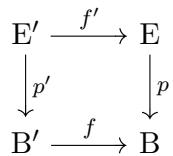
\includegraphics[keepaspectratio]{images/part001_2db9b8ac.jpg}}

为一个笛卡尔方块。设 B-空间 (E, p) 是覆叠，且空间 B' 是连通且局部连通的。设 b' 为 B' 的一点。B'-空间 (E', p') 是可平凡化覆叠，当且仅当对 E 的每个满足 \(p(x) = f(b')\) 的点 x，存在 f 的连续提升 \(g: B' \to E\)，使得 \(g(b') = x\)。

回忆 \((\mathrm{E}^{\prime}, p^{\prime})\) 是 \(B^{\prime}\) 的覆叠 (I, p. 71, cor. 2)，且映射 \(f^{\prime}\) 诱导双射 \(E_{b^{\prime}}^{\prime} \to E_{f(b^{\prime})}\) (I, p. 10, cor.)。由 I, p. 9 的 prop. 3，映射 \(s \mapsto f^{\prime} \circ s\) 定义了 \(p^{\prime}\) 的连续截面所成之集与 f 到 E 中的连续提升所成之集之间的一个双射。于是该推论由推论 4 得出。

命题 7. --- 设 B 为拓扑空间，E 与 E' 为 B-空间，f: E' → E 为 B-态射。设 E' 是 B 的覆叠且空间 B 是局部连通的。

\begin{enumerate}
\def\labelenumi{\alph{enumi})}
\item
  若 B-空间 E 的投影是平展且分离的映射，则 \((\mathrm{E}^{\prime}, f)\) 是 E 的覆叠。
\item
  若 f 是满的，则 E 是 B 的覆叠。
\end{enumerate}

用 \(p\) 与 \(p'\) 分别表示 B-空间 E 与 E′ 的投影。在假设 \(a\) 之下，\(f\) 是平展的 (I, p. 29, prop. 6, c))。在假设 \(b\) 之下，\(p\) 是平展的（同处 d)）。因此，在这两个假设的任一个之下，E 都是局部连通的；其连通分支特别在 E 中既开又闭 (TG, I, p. 85, prop. 11)。

我们先在附加假设——B 是连通且局部连通的，而 E' 是平凡覆叠 (B × F', pr₁)——之下证明命题 7。

引理. --- 若 U 是 E' 的一个连通分支，则 f 在 U 上的限制诱导 U 到 E 的某个连通分支上的同胚。

设 \(x \in F'\) 使得 \(U = B \times \{x\}\) （参看 I, p. 79）。把 \(b \in B\) 映为 \(f(b, x)\) 的从 B 到 E 中的映射是 p 的连续截面。其像 X 因而是连通的且在 E 中是开的，因为 p 是平展的 (I, p. 30, cor. 3)。而且在假设 a) 之下它还是闭的，因为 p 是分离的 (I, p. 27, prop. 3)。在假设 b) 之下它也是闭的，由 I, p. 80 的推论 1，因为 U 在 E' 中既开又闭。于是 X 是 E 的一个连通分支。

由于 \(f \mid \mathrm{U} \colon \mathrm{U} \to \mathrm{X}\) 是双射且是开的，它是到其像上的同胚，这就证明了引理。

保留引理前面的假设，现在来证明断言 \(a\) )。设 V 为 E 的一个连通分支。它是 E 中的既开又闭集，而 \(f^{-1}(\mathrm{V})\) 是 \(\mathrm{E}'\) 的若干连通分支的并，由引理，\(f\) 把这些分支同胚地映到 V 上。由 I, p. 79 的 prop. 6 得出 \((\mathrm{E}', f)\) 是覆叠。

来证明 b)。由于 f 是满的，由引理得出 E 的每个连通分支 V 都是某个连通分支 \(U = B \times \{x\}\) （\(E'\) 的）的同胚像。于是映射 p 诱导 V 到 B 上的同胚。由 prop. 6，E 是 B 的覆叠。

这就在附加假设——B 是连通的且 E' 是 B 的可平凡化覆叠——之下证明了命题。来证明一般情形。

存在 B 的由连通开集组成的覆叠 \((\mathrm{U}_{i})_{i\in\mathrm{I}}\)，覆叠 \(E'\) 在这些开集上均可平凡化。设 \(i\in I\) 。

来证明 \(a\)。若映射 \(p\) 是平展且分离的，则映射 \(p_{\mathrm{U}_i}\colon \mathrm{U}_i\times_{\mathrm{B}}\mathrm{E}\to \mathrm{U}_i\) （对 \(i\in \mathrm{I}\)）同样如此，这由 I, p. 31 的 prop. 8 与 I, p. 27 的 prop. 4 得出。于是由已处理的特殊情形得出，对每个 \(i\in \mathrm{I}\)，\(\mathrm{U}_i\)-空间 \((\overline{p'}^{1}(\mathrm{U}_i),f_{\mathrm{U}_i})\) 是覆叠。用 A 表示不交并 \(\coprod_{i\in I}\mathrm{U}_i\) 的全空间，用 \(q\colon \mathrm{A}\to \mathrm{B}\) 表示典范映射。于是，空间 \(\mathrm{A}\times_{\mathrm{B}}\mathrm{E}'\) （赋以映射 \(f_{\mathrm{A}}\colon \mathrm{A}\times_{\mathrm{B}}\mathrm{E}'\to \mathrm{A}\times_{\mathrm{B}}\mathrm{E}\) 的）是 \(\mathrm{A}\times_{\mathrm{B}}\mathrm{E}\) 的覆叠。映射 \(q\) 在 B 的每一点的邻域内都有连续截面，而把 I, p. 72 的命题 3 应用于笛卡尔方块

\[
\begin{array}{c} \mathrm {A\times_ {B} E^ {\prime}} \longrightarrow \mathrm {E^ {\prime}} \\ \Big \downarrow f _ {\mathrm{A}} \\ \mathrm {A\times_ {B} E} \longrightarrow \mathrm{E} \end{array} ,
\]

蕴含 \(E'\) 是 E 的覆叠。

来证明 \(b\)。设 \(f\) 是满的。于是对 I 的每个元素 \(i\)，映射 \(f_{\mathrm{U}_i}\colon \mathrm{U}_i\times_{\mathrm{B}}\mathrm{E}'\to \mathrm{U}_i\times_{\mathrm{B}}\mathrm{E}\) 是满的，且空间 \(\mathrm{U}_i\times_{\mathrm{B}}\mathrm{E}'\) （赋以映射 \(f_{\mathrm{U}_i}\) 的）是 \(\mathrm{U}_i\times_{\mathrm{B}}\mathrm{E}\) 的覆叠 (I, p. 71, cor. 2 of prop. 2)。由前面处理的特殊情形得出，\(\mathrm{U}_i\)-空间 \((\overline{p}^{1}(\mathrm{U}_{i}),p_{\mathrm{U}_{i}})\) 是覆叠。从而 E 是 B 的覆叠。

设 B 为拓扑空间，E 与 E′ 为 B 的覆叠，\(f: E \rightarrow E'\) 为 B-态射。我们已经看到，在下列两个假设的每一个之下，\((E, f)\) 都是覆叠：1) 覆叠 E 是局部有限次的 (I, p. 76, cor. 1)；2) 空间 B 是局部连通的 (I, p. 81, prop. 7)。这一现象可以解释如下。

设 F 与 F′ 为离散拓扑空间，\(f: B \times F \to B \times F'\) 为 B-态射。由 \(\widetilde{f}: b \mapsto \mathrm{pr}_{2} \circ f(b, \cdot)\) 给出的从 B 到空间 \(\mathcal{C}_{c}(F; F')\) 中的映射是连续的 (TG, X, p. 28, th. 3)。若 U 是 B 的开子集且映射 \(\widetilde{f}\) 在 U 上是常值的，则由 f 诱导出的映射 \(f_{U}: U \times F \to U \times F'\) 是可平凡化覆叠 (I, p. 69, prop. 1)。

空间 \(\mathcal{C}_c(\mathrm{F};\mathrm{F}')\) 无非就是映射所成之集 \(\mathcal{F}(\mathrm{F};\mathrm{F}')\) （从 F 到 \(\mathrm{F}'\) 中的），赋以经由典范同构由积空间 \((\mathrm{F}')^{\mathrm{F}}\) 的拓扑所诱导的拓扑。对这个拓扑，空间 \(\mathcal{F}(\mathrm{F};\mathrm{F}')\) 是全不连通的 (I, p. 84, prop. 10)。于是，若空间 B 是连通的，则映射 \(\widetilde{f}\) 是常值的 (I, p. 82, prop. 4)；若空间 B 是局部连通的，则映射 \(\widetilde{f}\) 是局部常值的。当集 F 有限时，空间 \(\mathcal{F}(\mathrm{F};\mathrm{F}')\) 是离散的，而映射 \(\widetilde{f}\) 是局部常值的。

注. --- 设 B 为拓扑空间，\((\mathrm{E}, p)\) 与 \((\mathrm{E}', p')\) 为 B-空间，\(f: E' \to E\) 为 B-态射。

\begin{enumerate}
\def\labelenumi{\alph{enumi})}
\item
  若 E 与 E' 是 B 的覆叠，则映射 f 是平展的 (I, p. 29, prop. 6) 且分离的 (I, p. 25, prop. 2)。但若空间 B 不是局部连通的，则一般而言 (E', f) 未必是 E 的覆叠 (I, p. 145, exerc. 4)。
\item
  若 \((\mathrm{E}^{\prime}, p^{\prime})\) 是 B 的覆叠，f 是满的且使 \(E^{\prime}\) 成为 E 的覆叠，则映射 p 是平展的 (I, p. 29, prop. 6)。但若空间 B 不是局部连通的，则一般而言它未必是分离的 (I, p. 145, exerc. 4)。特别地，E 未必是 B 的覆叠。
\end{enumerate}

推论. --- 设 B 为连通且局部连通的拓扑空间。设 E 与 E' 为 B 的覆叠。设 b 为 B 的一点。设 \(f: E' \to E\) 为 B-态射，\(f_{b}: E_{b}' \to E_{b}\) 为 f 通过限制到纤维上所诱导的映射。若映射 \(f_{b}\) 是单射（相应地，满射，相应地，双射），则映射 f 亦然。

用 \(p\) 表示 B-空间 E 的投影。由该命题，\((\mathrm{E}', f)\) 是 E 的覆叠；其像 \(f(\mathrm{E}')\) 在 E 中既开又闭。用 U 表示 \(f(\mathrm{E}')\) 在 E 中的补集，于是 B-空间 \((\mathrm{U}, p \mid \mathrm{U})\) 是 B 的覆叠 (I, p. 80, corollary 1)。若映射 \(f_b\) 是满的，则这个覆叠在 \(b\) 处的纤维是空的。由于 B 是连通空间，这时 U 是空的，故 \(f\) 是满的。

E 中使 f 的纤维恰含一个元素的点所成的集 V 是既开又闭的。B-空间 \((V, p|V)\) 与 \((f(E'), p|f(E'))\) 是 B 的覆叠（同处），且典范映射 \(i: V \to f(E')\) 是 B-态射。若映射 \(f_b\) 是单射，则映射 \(i_b\) 是满的，故由前述结果 i 是满的，从而 \(V = f(E')\)。于是映射 f 是单射。

